\documentclass[a4paper,oneside]{memoir}

\setlength{\trimtop}{0pt}
\setlength{\trimedge}{\stockwidth}
\addtolength{\trimedge}{-\paperwidth}
\settypeblocksize{24cm}{14cm}{*}
\setulmargins{3cm}{*}{*}
\setlrmargins{3.5cm}{*}{*}
\setmarginnotes{17pt}{51pt}{\onelineskip}
\setheadfoot{\onelineskip}{2\onelineskip}
\setheaderspaces{*}{2\onelineskip}{*}
\checkandfixthelayout

\clubpenalty = 10000 
\widowpenalty = 10000 
\displaywidowpenalty = 10000

\usepackage{selinput}
\usepackage{microtype}
\usepackage{graphicx}
\usepackage{hyperref} % muss letztes package sein

\hypersetup{pdfborder=0 0 0}

\title{Designing a Real KERNAL Cartridge}
\author{
Thomas 'skoe' Giesel
(skoe@directbox.com)
}

\begin{document}
\emergencystretch=0.15\hsize

%%%%%%%%%%%%%%%%%%%%%%%%%%%%%%%%%%%%%%%%%%%%%%%%%%%%%%%%%%%%%%%%%%%%%%%%
\pagestyle{empty}
\begin{center}

\vspace*{5cm}
\textsc{\huge Designing a Real KERNAL Cartridge}\\[2cm]
{\large Thomas 'skoe' Giesel}

\vfill

% Bottom of the page
{\large Version 1.1 \\[0.5cm] \today}

\end{center}
%%%%%%%%%%%%%%%%%%%%%%%%%%%%%%%%%%%%%%%%%%%%%%%%%%%%%%%%%%%%%%%%%%%%%%%%

\clearpage

\tableofcontents

\chapter{Introduction}

\section{The Need for a KERNAL Cartridge}

Nearly all Commodore computers contain a KERNAL ROM. The KERNAL ROM
contains the operating system of the machine, providing the drivers
necessary for low level input/output access, among other functions.
However, since the KERNAL is a ROM and cannot be easily modified, it
can be hard to upgrade the functionality in the KERNAL.

On the Commodore 64, the KERNAL is used to access the serial bus and
therefore the disk drives. Most often, people look to KERNAL
upgrades to address slow disk access issues. The standard KERNAL
drivers in the C64 offer only slow transfer functionality, while
there are many replacement KERNAL offerings that allow greatly
enhanced transfer functionality. However, this is not the only
reason a KERNAL replacement might be desired. Auto-boot
functionality, customized screen layout, or other reasons might
demand a KERNAL replacement.

While there are alternative ways to
replace some KERNAL functionality, those mechanisms limit
usefulness. Changing KERNAL vectors that are located in RAM only
applies to callers that utilize those vectors, and only vectorized
functionality can be enhanced. As well, new functionality must
exist in the address space, which might conflict with application
code. Thus, cartridges like Action Replay, Fastload, or The Final
Cartridge III cannot always offer the level of compatibility
desired.

One well-known replacement KERNAL is JiffyDOS. To use JiffyDOS, one
must replace the KERNAL ROM in the host machine with a new ROM,
while the operating system of each drive must be upgraded as well.
Though, some drives, like CMD devices and sd2iec-based devices,
support JiffyDOS standard.

Disk drives typically socket their DOS ROM, for easy replacements.
However, many computer systems do not socket the KERNAL ROM, making
replacement much harder.

A KERNAL cartridge can address these issues. The cartridge would
allow the same functionality as a KERNAL replacement, but would not
require disassembly of the computer system or soldering of a socket
to the circuit board to allow replacement.

\section{KERNAL Cartridge Design Challenges}

When not in "Ultimax" mode, which radically changes the memory map
to mimic the layout in the Commodore Ultimax system, the KERNAL can
be found in the C64 address space at \$E000 to \$FFFF, an 8KiB
section of memory.
But the KERNAL is not the only memory in this address space.
There is also RAM below the KERNAL.
Programs can decide if they want to read the KERNAL ROM or the RAM there by
setting the HIRAM bit in the I/O register \$01 of the 6510 CPU.
Figure \ref{fig:memory-map-plain} shows the memory map of the C64
with no cartridge attached.

\begin{figure}
    \centering
    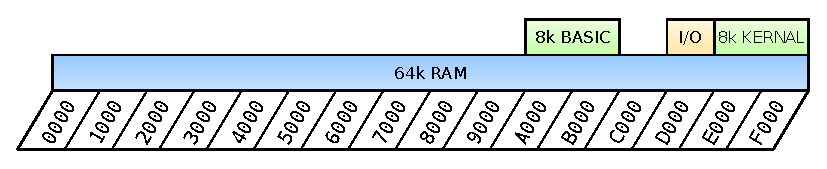
\includegraphics[width=15cm]{src/memory-map-plain}
    \caption{Memory map of the C64 with no cartridge attached}
    \label{fig:memory-map-plain}
\end{figure}

Write accesses from the CPU are always done to the RAM below the
KERNAL. The VIC-II always reads from that RAM but not from the KERNAL
ROM. But CPU read accesses depend from the signal \#HIRAM, which is
set in bit 1 of the I/O register \$01. If \#HIRAM is low (0), RAM
is read. If it is high (1), KERNAL ROM is read. Figure \ref
{fig:memory-map-hiram} shows this mechanism.

\begin{figure}
    \centering
    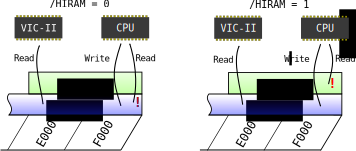
\includegraphics[width=11cm]{src/memory-map-hiram}
    \caption{\#HIRAM controls access to KERNAL memory space}
    \label{fig:memory-map-hiram}
\end{figure}

A compatible KERNAL cartridge must implement this behavior.
Otherwise, programs which use \$01 to hide the KERNAL ROM will fail,
because they cannot use the RAM between \$E000 and \$FFFF. However,
the \#HIRAM signal is not available on the Expansion Port. That is why
many KERNAL cartridges either do not provide access to this RAM area
or have to use a wire which must be connected to the \#HIRAM signal
inside the C64.

For a compatible KERNAL cartridge with no additional wire, the
cartridge must use another method to determine the state of \#HIRAM.
Since a write to address \$01 sets the state of \#HIRAM, one obvious
idea involves tracking any writes to \$01. However, writes to \$00
and \$01 do not present data on the C64 data bus, rendering such a
solution ineffective.

\chapter{KERNAL Cartridge Design}

\section{Working principle}

\#HIRAM does not act alone in re-arranging the memory map. Two lines
on the expansion port, \#GAME and \#EXROM, also play a part in
configuring it.

Pulled up via resistors inside the C64, these two lines can be configured via an external cartridge.
When there is no cartridge attached, both of them are high (1).
When a cartridge is attached, it can pull one or both of these lines low (0) to change the memory configuration. 
In this case, the memory configuration can still be changed with the 6510 I/O port, e.g.,
to hide the cartridge ROM.

There are two more control lines on the Expansion 
Port\footnote{In fact there are even more, but these two are interesting now.}:
\#ROML and \#ROMH. Excepting Ultimax mode, \#ROML selects an external
cartridge ROM into \$8000-\$9FFF, while \#ROMH selects a ROM into
\$A000-\$BFFF. Whenever the C64, via the address mapping logic in
the Programmable Logic Array (PLA), decides that data from a
cartridge must be read, it pulls down one of these lines.
Traditionally they are connected directly to two 8 KiB ROM ICs in
the cartridge.

An example: A cartridge pulls down \#GAME and \#EXROM to tell the C64
that there is a 16 KiB cartridge attached. The currently running
program has not disabled ROM by leaving \#HIRAM and \#LORAM as 1. When
the program wants to read a byte at \$A123, which is in the upper
cartridge ROM, the PLA determines that this byte must be read from
the external cartridge and brings \#ROMH active (0).

Table \ref {tab:game-exrom} shows the configurations which can be set by a cartridge using \#GAME and \#EXROM.

\begin{table}
    \centering
    \begin{tabularx}{\textwidth}{ccX}
        \toprule
        GAME & EXROM & Memory Map \\
        \midrule
        1 & 1 & No cartridge attached, memory map unchanged \\[3pt]
        1 & 0 & 8 KiB cartridge, \#ROML mapped to \$8000..\$9FFF \\[3pt]
        0 & 0 & 16 KiB cartridge, \#ROML mapped to \$8000..\$9FFF, \#ROMH mapped to \$A000..\$BFFF \\[3pt]
        0 & 1 & Compatibility mode to Commodore MAX, Ultimax mode,
                \#ROML mapped to \$8000..\$9FFF, \#ROMH mapped to \$E000..\$FFFF \\[3pt]
        \bottomrule
    \end{tabularx}
    \caption{Configurations of \#GAME and \#EXROM}
    \label{tab:game-exrom}
\end{table}

In \cite[Appendix~A]{PLA12} several different memory configurations are described.
Some interesting cases are shown in table \ref {tab:mem-configs}.
In configurations (1), (2) and (3) no cartridge is attached, i.e., \#GAME and \#EXROM are 1.
Only \#HIRAM controls whether there is RAM or KERNAL ROM visible to the CPU at \$E000 in these cases.

\begin{table}
    \begin{tabularx}{1.04\textwidth}{ccccccc}
        \toprule
        Config & \#LORAM & \#HIRAM & \#GAME & \#EXROM & \$A000..\$BFFF & \$E000..\$FFFF \\[3pt]
        (1)    & 1       & 1       & 1      & 1       & BASIC          & KERNAL \\[3pt]
        (2)    & x       & 0       & 1      & 1       & RAM            & RAM    \\[3pt]
        (3)    & 0       & 1       & 1      & 1       & RAM            & KERNAL \\[3pt]
        \midrule
        (4)    & x       & 1       & 0      & 0       & ROMH           & KERNAL \\[3pt]
        (5)    & 0       & 0       & 0      & 0       & RAM            & KERNAL \\[3pt]
        (6)    & 1       & 0       & 0      & 0       & RAM            & RAM    \\[3pt]
        \midrule
        (7)    & x       & x       & 0      & 1       & ---            & ROMH   \\[3pt]
        \bottomrule
    \end{tabularx}
    \caption{Memory configurations}
    \label{tab:mem-configs}
\end{table}

There is also a memory area controlled by \#HIRAM, which results in a
control signal visible at the Expansion Port: When a 16 KiB
cartridge is attached to the Expansion Port, \#HIRAM is used to
select whether the \#ROMH part of the cartridge or the internal RAM
is mapped to \$A000. This is shown in configurations (4), (5) and (6).

This proves invaluable for external KERNAL cartridge design. If the
cartridge sets the \#GAME and \#EXROM lines low, and a read
access of \$A000-\$BFFF occurs, \#ROMH provides the state of
\#HIRAM. As \#ROMH is connected to the Expansion Port, it can be
captured by the cartridge.

However, the cartridge needs to know the state of \#HIRAM during 
accesses to \$E000-\$FFFF, not \$A000-\$BFFF. The KERNAL
cartridge must force an access to \$A000-\$BFFF, but it cannot
change any running application code. Given those requirements, the
cartridge must find a way to drive the address bus itself in a way
that does not affect the running application.

When the CPU wants to read something, it sets its address outputs to
the address to be read. This address must be altered by the KERNAL 
cartridge to detect the state of \#HIRAM. But this must be done 
carefully, because it fights against the CPU address
line drivers and could overheat them when being used excessively.

The 6510 CPU has the ability to turn off its address line
drivers, via a control input called Address Enable Control (AEC). If
this input is low, the CPU effectively deactivates the address line
drivers. AEC is not connected to the Expansion
Port directly. But it is driven by the \#DMA signal, which is
available on the Expansion Port. Unfortunately, \#DMA also changes
the state of another CPU control line, Ready (RDY), which will stop
the CPU.

The 6500 CPU family datasheet shows that when RDY is asserted during a Phi2 cycle and released before the cycle ends, 
it should be ignored and should not stop the CPU. 
Thus, it seems like if the cartridge asserts \#DMA during a Phi2 cycle but releases it before the cycle ends, it could drive the address bus during that cycle.
This mechanism was tested on different C64 models. 
It turned out that some machines got unstable and crashed occasionally.
Obviously, the use of the RDY line as described above renders the CPU unstable.

Fortunately, a method was found which does not involve \#DMA.
Whenever a CPU read access to the address range \$F000-\$FFFF is detected, 
the cartridge pulls down the address line A14 for a fraction of the clock cycle.
This changes any address between \$F000-\$FFFF to an address between \$A000-\$BFFF.
After this is done, the state of \#HIRAM can be read from \#ROMH.

If the CPU accesses the KERNAL ROM, the cartridge must place the external KERNAL ROM into the address space at \$E000-\$FFFF.
The memory map shows a way to accomplish that.
Configuration (7) in table \ref {tab:mem-configs} illustrates "Ultimax" mode.
In this mode, any read access in the range \$E000-\$FFFF will activate the \#ROMH signal and will read from external memory.
Therefore, if a valid KERNAL read access is requested, the cartridge must set \#GAME to active (0) and release \#EXROM.
If RAM is to be read instead, the cartridge releases all lines to allow an ordinary RAM access.
When the Phi2 cycle ends, the cartridge releases all lines in any case to return to idle state.

The whole procedure is shown in figure \ref {fig:working-principle}. Note that also the signal BA must be evaluated, to distinguish a CPU read access from a VIC-II read access. As the VIC-II always reads from RAM but never from KERNAL, the mechanism must ignore read accesses by the VIC-II.
 
\begin{figure}
    \centering
    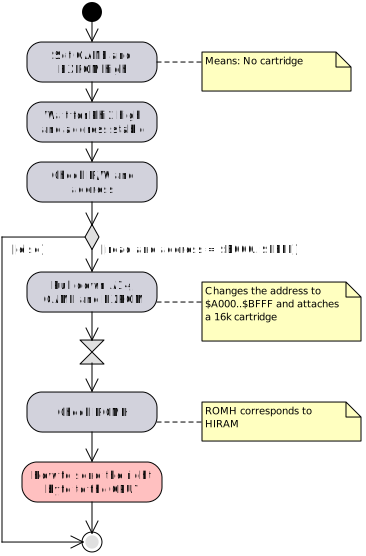
\includegraphics[width=10cm]{obj/working-principle}
    \caption{Working principle (simplified)}
    \label{fig:working-principle}
\end{figure}

\section{Optimization}

\label{sec:optimization}As mentioned already, write accesses to the CPU I/O register \$01 and the data direction register \$00 can be detected on the address bus and the R\#W line.
The only thing missing is the actual data byte written there. 
The cartridge utilizes this fact for an optimization.
The \#HIRAM detection is not done for every cycle when the CPU reads KERNAL space.
Instead, it only needs to be detected once, when the KERNAL address space is read the first time after \$00 or \$01 have been written.
For all additional CPU read accesses at this address range, the previously detected state of \#HIRAM is used, which significantly reduces the bus traffic, especially on the address line A14.

\section{Timing Considerations}

\label{sec:timing}Some of the steps needed for the external KERNAL implementation have
to consider timing requirements of the components of the C64. 
Most of them can be found in datasheets.

When Phi2 goes high, the VIC-II sets AEC high when it wants to allow a
CPU cycle. After this signal reached the CPU, it brings the address bus to the final value. 
The signals RAS and CAS by the VIC-II are used to set up the address into the DRAM chips.
CAS ends $T_{CHL} \le 220 ns$ after Phi2, according to \cite{VICII}.
CAS is further delayed by approximately 35 ns by the PLA, resulting in the signal CASRAM\footnote{The datasheet of the Signetics 82S100 PLA \cite{Si75} specifies a typical
propagation delay TPD of 35 ns and a maximum delay of 80 ns. The
Sharp custom IC used in newer C64s has different timings for
different output lines, but in the same ballpark. None of them actually needs 80 ns under normal conditions, as shown in \cite{PLA12}}.
This means that the addresses need to remain stable for this time plus the address hold time of the DRAMs, which is typically 10 ns to 20 ns.

This means that the external KERNAL cartridge must not modify the address bus less than 280 ns after the rising edge of Phi2.
At this time it sets \#GAME, \#EXROM and A14.
To hide the latency of the flash memory used on the cartridge, it starts a speculative read of the KERNAL memory content at this address.
The resulting data byte is prepared in the external KERNAL cartridge, but only put onto the C64's data bus when \#ROMH gets low, which happens asynchronously about 35 ns after A14 has been modified,   which is about 315 ns after the rising edge of Phi2.
The results in enough time for the the Data Stability Time Period ($T_{DSU} \ge 100 ns$) for the 6510 data lines. 

The PLA output is evaluated by the cartridge 80 ns after having set all input conditions.
This is also the time when the cartridge releases A14 and \#EXROM if it is a KERNAL access, and all lines if it is a RAM access. This happens about 360 ns after Phi2.

Even though the timing is very tight, it conforms to the values listed in the datasheets.
Also in real world it proofed to work reliable, as shown in section \ref{sec:ef3}.

All times measured by the cartridge are implemented as multiples of 40 ns.
A CPLD with a 25 MHz clock is used for that.
As the C64 signals come from another clock domain, up to 40 ns may be added to the times relative to Phi2 described above.
Figure \ref {fig:timing} shows the expected timing including the worst case addition of 40 ns.

\begin{figure}[!hb]
    \centering
    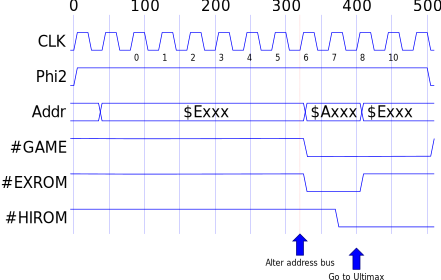
\includegraphics[width=10cm]{obj/implemented-timing}
    \caption{Timing of the External KERNAL Cartridge (worst case)}
    \label{fig:timing}
\end{figure}

\chapter{Actual Implementation}

\section{EasyFlash 3}

\label{sec:ef3} The multi-function cartridge EasyFlash~3 contains a KERNAL implementation based on this document, among other cartridge modes.
The cartridge contains flash memory, SRAM, a 25~MHz clock source, a 144 macrocell CPLD and a USB device interface for data connections to PCs.

The hardware design files are released under the Creative Commons license CC~BY-SA~3.0.
They are available at the public repository
\url{https://bitbucket.org/skoe/easyflash/src/tip/Hardware/ef3-kicad/}.

The CPLD core implemented in VHDL is licensed under the zlib license.
It is also available in that repository:
\url{https://bitbucket.org/skoe/easyflash/src/tip/Hardware/ef3-vhdl}.
The file \texttt{Hardware/ef3-vhdl/architecture.txt} in the repository contains a
detailed description of the implementation.

Figures \ref{fig:ef311} and \ref{fig:ef313} show two versions of the EasyFlash 3.

\begin{figure}[!h]
    \centering
    \includegraphics[width=10cm]{src/ef3-1-1}
    \caption{EasyFlash 3, short version}
    \label{fig:ef311}
\end{figure}

\section{Implemented Timing}

A logic analyzer was used to capture the signals from an EasyFlash~3 to verify the correct implementation and to compare it to the theory. 
The implementation corresponds to the description given in section \ref{sec:timing}. Figure \ref{fig:la-detect} shows a cycle with a \#HIRAM detection, followed by a read access to the external KERNAL. Figure \ref{fig:la-read} shows a read access from the external KERNAL without a \#HIRAM detection. In this case a previously detected \#HIRAM state was used, as described in section \ref {sec:optimization}.

\begin{figure}[!h]
    \centering
    \includegraphics[width=1.1\textwidth]{obj/la-detect}
    \caption{HIRAM Detection Captured with a Logic Analyzer}
    \label{fig:la-detect}
\end{figure}

\begin{figure}[!h]
    \centering
    \includegraphics[width=1.1\textwidth]{obj/la-read}
    \caption{Read Access Captured with a Logic Analyzer}
    \label{fig:la-read}
\end{figure}

\section{Compatibility}

As the time of writing, there are at least 500 EasyFlash~3 cartridges out there, sold by different vendors and built by several hobbyists.
There were many confirmations that the feature works reliable but no negative feedback.
It does not work on the Commodore 128 because it uses a completely different circuitry.
A few very early C64s have issues, because their reset line is driven with a push-pull output, which interferes with the external reset.

\begin{figure}[!h]
    \centering
    \includegraphics[width=7cm]{src/ef3-1-3}
    \caption{EasyFlash 3, long version}
    \label{fig:ef313}
\end{figure}

\begin{thebibliography}{999}

\bibitem [Si75]{Si75} Signetics, 1975, part of \textit{Mos and Bipolar ROM / PROM 1975}
\url{http://www.datasheetarchive.com/82S100-datasheet.html}.

\bibitem [PLA12]{PLA12} Thomas 'skoe' Giesel, 2012, \textit{The C64 PLA Dissected},
\url{http://skoe.de/docs/c64-dissected/pla/}.

\bibitem [VICII]{VICII} Commodore Semiconductor Group, \textit{6567 Video Interface Chip Specification Sheet}.

\end{thebibliography}



\end{document}

